\section{Risk-Neutral Policy Gradient Theorem}
In the previous sections, we saw that the core of a policy gradient algorithm consist in the approximation of the objective function gradient. In this section we present the \emph{policy gradient theorem} \cite{sutton1999policy}, which shows that the gradient can be rewritten in a form suitable for estimation from experience aided by an approximate action-value or advantage function. First, we will prove the theorem in the risk-neutral setting for which it was originally proposed. In particular, we will see how the GPOMDP algorithm can be easily derived by this result via a Monte Carlo approximation. Moreover, we will derive a class of actor-critic algorithms \cite{konda1999actor} that, in addition to a parametric approximation of the policy, also exploit an approximation of the action-value function or of an advantage function to reduce the variance of the gradient estimate. In particular, we review the powerful idea of compatible function approximation \cite{sutton1999policy} which assures the convergence to a local optimum of the objective function. Finally, we discuss the natural policy gradient idea \cite{kakade2001natural}, which forms the basis of many state-of-the-art algorithms. The extension to the risk-sensitive setting will be done in the next section. 

\subsection{Theorem Statement and Proof}
\begin{theorem}[Risk-Neutral Policy Gradient]
\label{thm:risk_neutral_policy_gradient}
	Let $\pi_\theta$ be a differentiable policy. The policy gradient for the average reward formulation is given by
	\begin{equation}
		\nabla_\theta \rho(\theta) =
		\E[\substack{S \sim d^\theta\\A \sim \pi_\theta}]{\nabla_\theta\log
		\pi_\theta(S,A) Q_{\theta}(S, A)}
	\end{equation}
	where $d^\theta$ is the stationary distribution of the Markov chain induced by $\pi_\theta$. The policy gradient for the start value formulation is given by
	\begin{equation}
		\nabla_\theta J_{\text{start}}(\theta) =
		\E[\substack{S \sim d_\gamma^\theta(s_0, \cdot)\\A \sim \pi_\theta}]{\nabla_\theta\log
		\pi_\theta(S,A) Q_{\theta}(S, A)}
	\end{equation}
	where $d_\gamma^\theta(s_0, \cdot)$ is the $\gamma$-discounted visiting distribution over states starting from the initial state $s_0$ and following policy $\pi_\theta$
		\begin{equation}
			d_\gamma^\theta(s, x) = \sum_{k=0}^{\infty} \gamma^k \calP_\theta^{(k)}(s, x)
		\end{equation}
\end{theorem}
\begin{proof}
	We first prove the result for the average-reward formulation and then for the start state formulation. From the basic relation between state-value function and action-value function, we have
	\begin{equation*}
		\begin{split}
			\nabla_\theta V_\theta(s) &= \nabla_\theta \int_{\A} \pi_\theta(s,a) Q_\theta(s,a) da\\
				&= \int_{\A} \left[ \nabla_\theta \pi_\theta(s,a) Q_\theta(s,a) + \pi_\theta(s,a) \nabla_\theta Q_\theta(s,a)\right] da
		\end{split}
	\end{equation*} 
	Using the Bellman expectation equation for $Q_\theta$ 
	\begin{equation*}
		\begin{split}
			\nabla_\theta Q_\theta(s,a) &= \nabla_\theta \left[ \calR(s,a) - \rho_\theta + \int_{\S} \calP(s,a,s') V_\theta(s') ds' \right]\\
			&= -\nabla_\theta \rho_\theta + \int_{\S} \calP(s,a,s') \nabla_\theta V_\theta(s') ds'
		\end{split}
	\end{equation*}
	Hence, plugging in the first equation 
	\begin{equation*}
		\begin{split}
			\nabla_\theta V_\theta(s) &= \int_{\A} \nabla_\theta \pi_\theta(s,a) Q_\theta(s,a) da - \nabla_\theta \rho_\theta + \int_\A \pi_\theta(s,a) \int_{\S} \calP(s,a,s') \nabla_\theta V_\theta(s') ds' 
		\end{split}
	\end{equation*} 	
	Integrating both sides with respect to the stationary distribution $d^\theta$ and noting that, because of stationarity,  
	\begin{equation*}
		\int_{\S} d^\theta(s) \int_{\A} \pi(s,a) \int_{\S} \calP(s,a,s') \nabla_\theta V(s') ds' da ds = \int_{\S} d^\theta(s) \nabla_\theta V_\theta(s) ds
	\end{equation*}
	we obtain the result 
	\begin{equation*}
		\begin{split}
		\nabla_\theta \rho_\theta &= \int_{\S} d^\theta(s) \int_{\A} \nabla_\theta \pi_\theta(s,a) Q_\theta(s,a) da ds\\
		&= \int_{\S} d^\theta(s) \int_{\A} \pi_\theta(s,a) \nabla_\theta \log\pi_\theta(s,a) Q_\theta(s,a) da ds\\
		&= \E[\substack{S \sim d^\theta\\A \sim \pi_\theta}]{\nabla_\theta\log
				\pi_\theta(S,A) Q_{\theta}(S, A)} 
		\end{split}
	\end{equation*}
	Let us now prove the theorem for the start state formulation. The first step is exactly the same. Hence, using the Bellman expectation equation for $Q_\theta$ 
	\begin{equation*}
		\begin{split}
			\nabla_\theta Q_\theta(s,a) &= \nabla_\theta \left[ \calR(s,a) + \gamma \int_{\S} \calP(s,a,s') V_\theta(s') ds' \right]\\ 
			&= \gamma \int_{\S} \calP(s,a,s') \nabla_\theta V_\theta(s') ds'
		\end{split}
	\end{equation*}
	we obtain
	\begin{equation*}
		\begin{split}
			\nabla_\theta V_\theta(s) &= \int_{\A} \left[ \nabla_\theta \pi_\theta(s,a) Q_\theta(s,a) + \gamma \int_{\S} \calP(s,a,s') \nabla_\theta V_\theta(s') ds' \right] da\\
			&= \int_\S  \sum_{k=0}^{\infty} \gamma^k \calP_\theta^{(k)}(s, x) \int_{\A} \nabla_\theta \pi_\theta(x,a) Q_\theta(x,a) da dx 
		\end{split}
	\end{equation*} 
	after unrolling $\nabla_\theta V_\theta$ infinite times and denoting by $\calP_\theta^{(k)}(s, x)$ the probability of going from state $s$ to state $x$ in $k$ steps under policy $\pi_\theta$.
	Defining the $\gamma$-discounted visiting distribution of state $x$ starting from state $s$ as
	\begin{equation*}
		d_\gamma^\theta(s, x) = \sum_{k=0}^{\infty} \gamma^k \calP_\theta^{(k)}(s, x)
	\end{equation*}
	we have the result
	\begin{equation*}
		\begin{split}
			\nabla_\theta V_\theta(s) &= \int_\S d_\gamma^\theta(s, x) \int_{\A} \nabla_\theta \pi_\theta(x,a) Q_\theta(x,a) da dx\\
			&= \E[\substack{S \sim d_\gamma^\theta(s_0, \cdot)\\A \sim \pi_\theta}]{\nabla_\theta\log \pi_\theta(S,A) Q_{\pi_\theta}(S, A)}
		\end{split}
	\end{equation*} 
\end{proof}
The action-value function is typically unknown and needs to be approximated. 
As for the REINFORCE algorithm, we can subtract a state-dependent baseline from the action-value function without changing the value of the expectation. Indeed 
\begin{equation*}
	\begin{split}
	\E[\substack{S \sim d^\theta\\A \sim \pi_\theta}]{\nabla_\theta\log
			\pi_\theta(S,A) B_\theta(S)} 
	&= \int_\S d^\theta(s) \int_\A \pi_\theta(s,a) \nabla_\theta\log
				\pi_\theta(s,a) B_\theta(s) da ds\\
	&= \int_\S d^\theta(s)  B_\theta(s) \int_\A \nabla_\theta \pi_\theta(s,a) da ds\\
	&= \int_\S d^\theta(s)  B_\theta(s)  \nabla_\theta  \underbrace{\int_\A  \pi_\theta(s,a) da}_{= 1} ds = 0
	\end{split}
\end{equation*}
Hence, we can rewrite the policy gradient for the average reward formulation as
\begin{equation}
\label{eq:pg_theorem_baseline}
	\nabla_\theta \rho(\theta) =
	\E[\substack{S \sim d^\theta\\A \sim \pi_\theta}]{\nabla_\theta\log
	\pi_\theta(S,A) \left(Q_{\pi_\theta}(S, A) - B_\theta(S)\right)}
\end{equation}
and similarly for the start state formulation. This result can be used as the starting point to derive several policy gradient methods that use different approximation of the action-value function. 

\subsection{GPOMDP}
For an episodic MDP, the action-value function can be estimated with the total return obtained on a sample trajectory
\begin{equation*}
	Q_\theta(s_0,a_0) \approx \sum_{t=0}^{T^{(m)}} \gamma^t r_{t+1}^{(m)}
\end{equation*}
Combining this remark with a Monte Carlo approximation of Eq. (\ref{eq:pg_theorem_baseline}), we obtain the GPOMDP gradient estimate (\ref{eq:GPOMDP}). Therefore, the GPOMDP algorithm is a simple application of the policy gradient algorithm, which is much more general than the likelihood ratio technique used to derive the algorithm in the previous sections. In the next subsections we present other ways to exploit the policy gradient theorem to design efficient learning algorithms.

\subsection{Actor-Critic Policy Gradient}
A baseline should ideally measure the typical return obtained by an agent in a certain state when following a certain policy. Therefore, it becomes natural to use the state-value function as a benchmark for the action-value function. Eq. (\ref{eq:pg_theorem_baseline}) thus becomes
\begin{equation}
\label{eq:actor_critic_pg}
	\nabla_\theta \rho(\theta) =
		\E[\substack{S \sim d^\theta\\A \sim \pi_\theta}]{\nabla_\theta\log
		\pi_\theta(S,A) A_\theta(S,A)}
\end{equation} 
where we introduced the advantage function
\begin{equation}
	A_\theta(s,a) = Q_\theta(s,a) - V_\theta(s)
\end{equation}
which measures how good is to take action $a$ in state $s$ compared to simply following the policy $\pi_\theta$. The advantage function is unknown and should estimated from samples of the MDP. \emph{Actor-Critic} algorithms consist in all those methods that employ an approximation of the advantage function or of the value function, also known as critic, to estimate the policy gradient. These methods thus maintain two sets of parameters: a \emph{critic} that updates the action-value function parameters $\psi$ and an \emph{actor} that updates the policy parameters $\theta$ in the direction suggested by the critic. The general structure for an online actor-critic algorithm is reported in Algorithm \ref{algo:actor_critic}.\\
\begin{algorithm}[t]
	\caption{Generic structure for an online actor-critic algorithm.}
	\label{algo:actor_critic}
	\begin{algorithmic}[0]
		\Require{\\
			\begin{itemize}
				\item Initial actor parameters $\theta_0$, 
				\item Initial critic parameters $\psi_0$, 
				\item Learning rate $\{\alpha_k\}$
			\end{itemize}
		} 
		\Ensure Approximation of the optimal policy $\pi_{\theta^*} \approx \pi_*$
		\begin{algorithmic}[1]
		\Repeat
			\State Observe tuple $<s_k, a_k, r_{k+1}, s_{k+1}>$ sampled from the MDP.
			\State Update critic parameters $\psi_{k+1}$ using a value-based method. 
			\State Estimate policy gradient as $\widehat{g}_k^\text{AC} = \nabla_\theta \log \pi_{\theta_k}(s_k, a_k) \widehat{A}_{\psi_{k+1}}(s_k, a_k)$
			\State Update actor by gradient ascent $\theta_{k+1} = \theta_k + \alpha_k \widehat{g}_k^\text{AC}$. 
			\State $k \leftarrow k + 1$
		\Until{converged}
		\end{algorithmic}
	\end{algorithmic}
\end{algorithm}
There are two possible approaches to estimate the advantage function: the first one is to estimate both the state-value function $\widehat{V}_\psi \approx V_\theta$ and the action-value function $\widehat{Q}_\xi \approx Q_\theta$ and derive an estimate for the advantage function $\widehat{A}_{\psi, \xi} = \widehat{Q}_\xi - \widehat{V}_\psi \approx A_\theta$. The second approach directly approximates the advantage function $\widehat{A}_\psi \approx A_\theta$ and is usually preferred, since it allows us to maintain only one critic. Actor-critic algorithms typically use a temporal-difference algorithm to update an approximation of the value function $\widehat{V}_\psi \approx V_\theta$, from which we can derive an approximation for the advantage function. Assume that the true state-value function $V_\theta$ is given. Then the TD error 
\begin{equation}
	\delta_\theta = R - \rho_\theta + V_\theta(S') - V_\theta(S)
\end{equation}
is an unbiased estimate of the advantage function. Indeed 
\begin{equation*}
	\begin{split}
		\E{\delta_\theta | S = s, A = a} &= \E{R - \rho_\theta + V_\theta(S') | S = s, A = a} - V_\theta(s)\\
		&= Q_\theta(s,a) - V_\theta(s)\\
		&= A_\theta(s,a)  
	\end{split}
\end{equation*}
By a simple conditioning argument, the policy gradient can be rewritten as
\begin{equation}
	\nabla_\theta \rho(\theta) =
			\E[\substack{S \sim d^\theta\\A \sim \pi_\theta}]{\nabla_\theta\log
			\pi_\theta(S,A) \delta_\theta}
\end{equation} 
In practice, we can use an approximate TD error 
\begin{equation}
\label{eq:td_error}
	\widehat{\delta}_k = r_{k+1} - \widehat{\rho}_k + \widehat{V}_{\psi_k}(s_{k+1}) - \widehat{V}_{\psi_k}(s_k) 
\end{equation}
where $\widehat{\rho}_k$ is an estimate of the average reward. Hence, we can easily obtain an approximation of the policy gradient by
\begin{equation}
	\widehat{g}_\text{TD(0)}^k = \nabla_\theta\log \pi_\theta(s_k,a_k) \widehat{\delta}_k
\end{equation}
which can be used to update the critic parameter in the gradient ascent direction. 
On the other hand, the critic parameters can be updated using a TD(0) temporal difference scheme
\begin{equation}
	\psi_{k+1} = \psi_k + \alpha_k \widehat{\delta}_k \nabla_\psi \widehat{V}_{\psi_k}(s_k)
\end{equation}
The discussion can be easily extended to more complex value-based methods for estimating the critic, such as the backward-view TD($\lambda$). This method employs eligibility traces to assign credit for the rewards obtained by the agent to all previous states and actions. More formally, the policy parameters update rule becomes
\begin{equation}
	\theta_{k+1} = \theta_k + \alpha_k \widehat{\delta}_k e_k
\end{equation}
where the eligibility trace $e_k$ is defined by the following recursive equation 
\begin{equation}
	e_{k+1} = \lambda e_k + \nabla_\theta\log \pi_{\theta_k}(s_k,a_k) 
\end{equation} 
$0 \leq \lambda \leq 1$ is a parameter that manages the amount of bootstrap: for $\lambda = 0$ the method is the standard temporal difference scheme while for $\lambda = 1$ the method is equivalent to Monte Carlo. The complete scheme is reported in Algorithm \ref{algo:actor_critic_td}. 
\begin{algorithm}[t!]
	\caption{TD($\lambda$) policy gradient algorithm.}
	\label{algo:actor_critic_td}
	\begin{algorithmic}[0]
		\Require{\\
			\begin{itemize}
				\item Initial actor parameters $\theta_0$, 
				\item Initial critic parameters $\psi_0$, 
				\item Learning rate $\{\alpha_k\}$
			\end{itemize}
		} 
		\Ensure Approximation of the optimal policy $\pi_{\theta^*} \approx \pi_*$
		\begin{algorithmic}[1]
		\State Initialize $k = 0$ and the eligibility trace $e_{-1} = 0$
		\Repeat
			\State Observe tuple $<s_k, a_k, r_{k+1}, s_{k+1}>$ sampled from the MDP.
			\State Compute TD error $\widehat{\delta}_k = r_{k+1} - \widehat{\rho}_k + \widehat{V}_{\psi_k}(s_{k+1}) - \widehat{V}_{\psi_k}(s_k) $
			\State Update critic parameters $	\psi_{k+1} = \psi_k + \alpha_k \widehat{\delta}_k \nabla_\psi \widehat{V}_{\psi_k}(s_k)$ 
			\State Update eligibility trace $e_{k+1} = \lambda e_k + \nabla_\theta\log \pi_{\theta_k}(s_k,a_k)$
			\State Update actor parameters $\theta_{k+1} = \theta_k + \alpha_k \widehat{\delta}_k e_k $. 
			
			\State $k \leftarrow k + 1$
		\Until{converged}
		\end{algorithmic}
	\end{algorithmic}
\end{algorithm}


\subsection{Compatible Function Approximation}
In the previous sections we saw that a critic may reduce the variance of thew policy gradient estimate. However, this is achieved at the cost of introducing a bias in the approximation which, in certain cases, may endanger the convergence of the method to a good solution. Luckily, the \emph{compatible function approximation}  \cite{sutton1999policy} avoids introducing any bias by a careful choice of the critic. This technique consists in estimating the advantage function with a linear regression on a family of suitable basis functions consisting of the gradient of the likelihood score, i.e.
\begin{equation}
	\widehat{A}_\theta (s,a) = \psi^T \nabla_\theta \log \pi_\theta(s,a)
\end{equation}
The power of these basis functions becomes apparent in the following theorem
\begin{theorem}[Compatible Function Approximation]
	If 
	\begin{enumerate}[label={\roman*)}]
		\item the advantage function approximator is compatible to the policy, i.e. 
		\begin{equation}
			\nabla_\psi A_\psi(s,a) = \nabla_\theta \log \pi_\theta(s,a)
		\end{equation}
		\item the advantage function parameters $\psi$ minimize the mean square error 
		\begin{equation}
			\theta = \argmin_\psi \E[\pi_\theta]{\left( A_{\pi_\theta}(S,A) - \widehat{A}_\psi(S,A)\right)^2}
		\end{equation}
	\end{enumerate}
	Then the policy gradient is exact
	\begin{equation}
		\nabla_\theta J(\theta) = \E[\pi_\theta]{\nabla_\theta \log \pi_\theta(S,A) \widehat{A}_\psi(S,A)}
	\end{equation}
\end{theorem} 
Hence, the true advantage function in the policy gradient formula can be replaced by the compatible function approximation without changing the policy gradient value. A linear regression may seem a too simple representation of the advantage function. However, one must bear in mind that this approximation is only used to reduce the variance of the policy gradient estimate and should not be expected to provide an accurate representation of the true-value function. This technique has proved useful in many application. 

\subsection{Natural Policy Gradient}
Despite all the advances in the variance reduction techniques, these methods still tend to perform surprisingly poorly. Even when applied to simple examples with rather few states, where the gradient can be determined very accurately, they turn out to be quite inefficient. Typically, one of the reasons of this behavior is the presence of large plateaus in the expected return landscape where the gradients are small and often do not point directly towards the optimal solution. In this context, the steepest ascent with respect to the Fisher information metric, called the \emph{natural policy gradient}, turns out to be significantly more efficient than normal gradients for such
plateaus. This technique was first proposed in the reinforcement learning setting in \cite{kakade2001natural} and later applied to actor-critic algorithms in in \cite{peters2008reinforcement}. The following properties of natural policy gradient make it one of the more reliable policy-based methods,
\begin{enumerate}[label={\roman*)}]
	\item Convergence to a local minimum is guaranteed.
	\item By choosing a more direct path to the optimal solution in parameter space, the natural gradient typically has faster convergence and avoids premature convergence of ``vanilla gradients''.
	\item  The natural policy gradient can be shown to be covariant, i.e. independent of the coordinate frame chosen for expressing the policy parameters.
	\item As the natural gradient analytically averages out the influence of the stochastic policy (including the baseline of the function approximator), it requires fewer data points for a good gradient estimate than ``vanilla gradients’'.
\end{enumerate}

\begin{figure}[!htb]
    \centering
    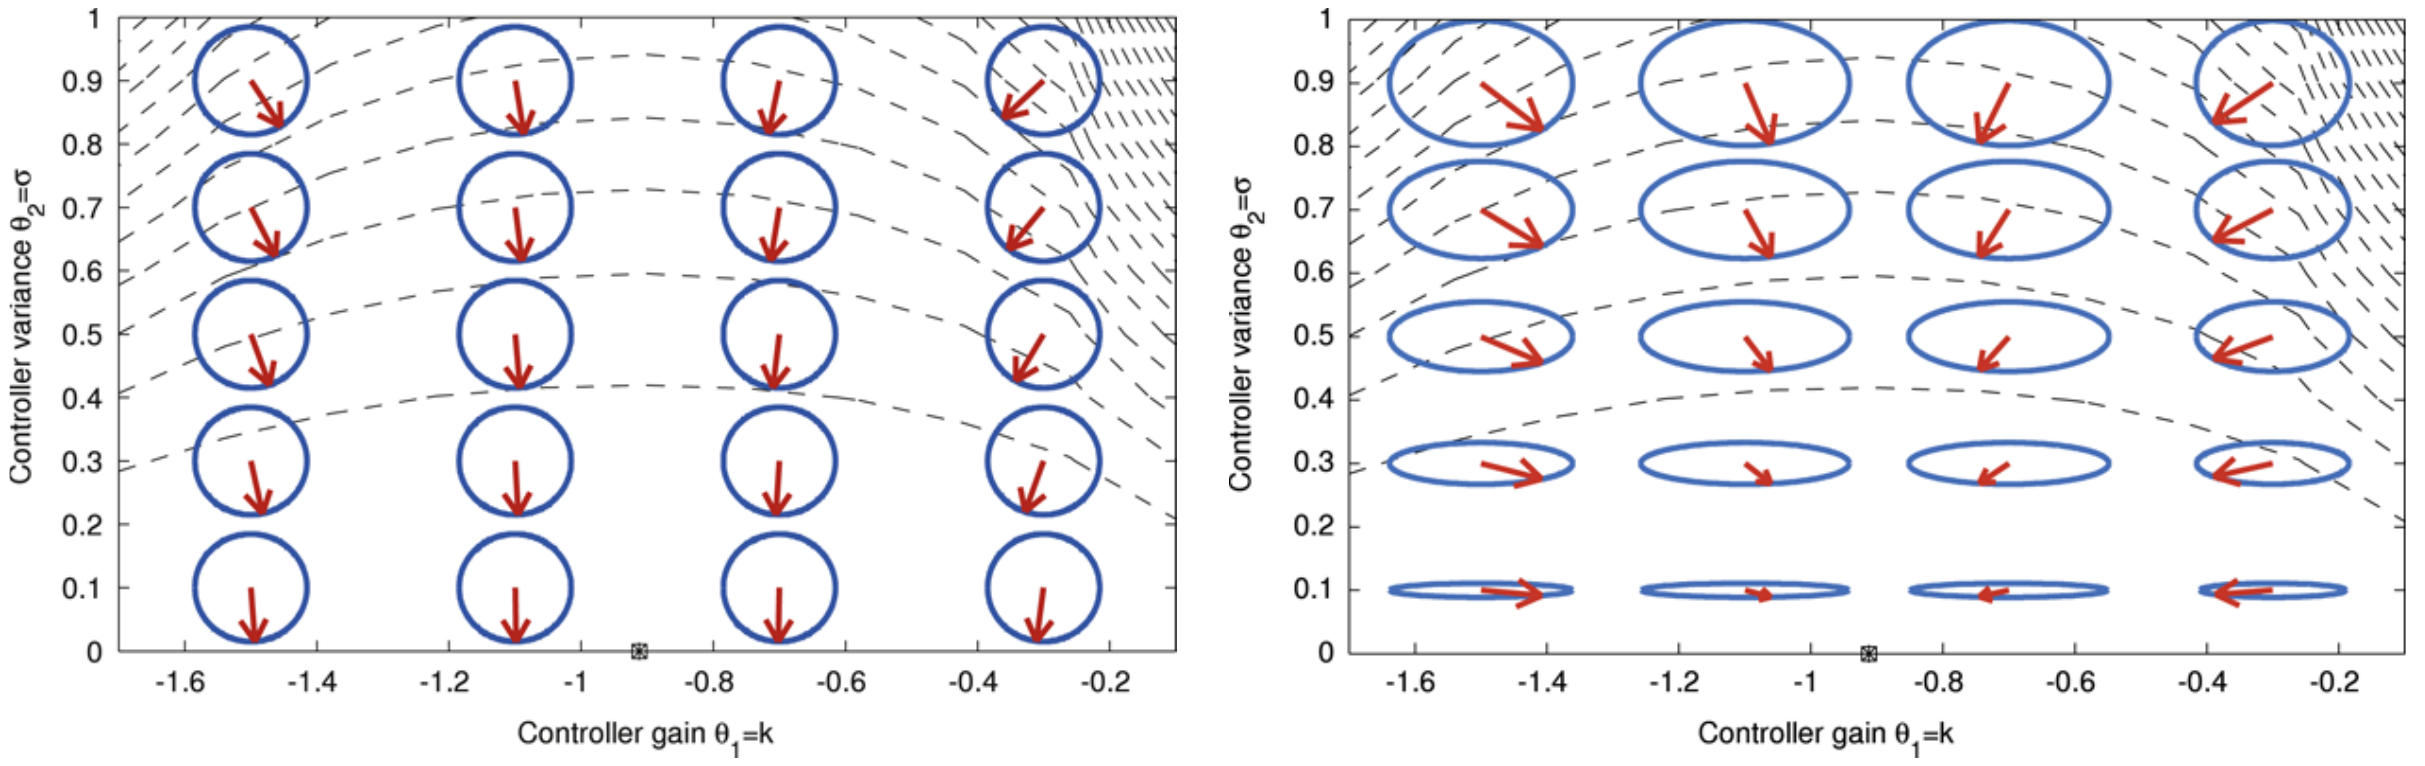
\includegraphics[width=1\linewidth]{Images/4_0_euclidean_vs_natural}
	\caption[``Vanilla'' policy gradient vs. natural policy gradient]{``Vanilla'' policy gradient (left) vs. natural policy gradient (right). The main difference is how the two approaches punish the change in parameters. This distance is 	indicated by the blue ellipses in the contour plot while the dashed lines show the expected return. Obtaining a gradient then corresponds to finding a vector pointing from the center of the ellipses to the location with maximum expected return on the ellipse. A vanilla policy gradient (a) considers a change in all parameters as equally distant, thus, it is a search for a maximum on a circle while the natural gradient (b) uses scales determined by the Fisher information which results in a reduction in exploration. The slower reduction in exploration results into a faster convergence to the optimal policy \cite{peters2008reinforcement}.}
\end{figure}

\subsubsection{Formalism of Natural Policy Gradients}
Policy gradient methods improve the policy $\pi_\theta$ by iteratively applying ``small'' changes $\Delta \theta$ to the policy parameters $\theta$. However, the meaning of ``small'' is ambiguous. For instance, when working with an Euclidean metric, the size of this update $\norm{\Delta \theta} = \sqrt{\Delta\theta^T \Delta\theta}$ and therefore the update size depends on the parameterization of the policy, which often results in unnaturally slow learning even if higher-order gradient methods were employed. This problem poses the question whether we can achieve a covariant gradient descent, i.e. a gradient descent with respect to an invariant measure of the closeness between the current policy and the updated policy based upon the distribution of the paths generated by each of these. Standard measures of distance between probability distributions are the Kullbach-Leibler divergence $d_{\text{KL}}(p_\theta(h)\ ||\ p_{\theta + \Delta \theta}(h))$ and the Hellinger distance. These two distances can be approximation in first instance by a second-order Taylor expansion
\begin{equation*}
	d_{\text{KL}}(p_\theta(h)\ ||\ p_{\theta + \Delta \theta}(h)) \approx \frac{1}{2} \Delta\theta^T F_\theta \Delta\theta
\end{equation*} 
where $F_\theta$ is the Fischer information matrix
\begin{equation}
	\begin{split}
	F_\theta &= \int_{\H} p_\theta(h) \nabla_\theta\log p_\theta(h) \nabla_\theta\log p_\theta(h)^T dh\\
		&= \E[H\sim p_\theta]{\nabla_\theta\log p_\theta(H) \nabla_\theta\log p_\theta(H)^T}
	\end{split}
\end{equation}
The goal is to find the optimal update $\Delta \theta$ for the policy parameters so as to maximize the objective function, under the constraint that the new policy must be in a radius $\epsilon$ from the previous policy with respect to the Kullbach-Leibler divergence, i.e.
\begin{equation*}
	\begin{cases}
		\max_{\Delta\theta} J(\theta + \Delta \theta) \approx J(\theta) + \Delta \theta^T \nabla_\theta J(\theta)\\
		\text{s.t.}\ d_{\text{KL}}(p_\theta(h)\ ||\ p_{\theta + \Delta \theta}(h)) \approx \frac{1}{2} \Delta\theta^T F_\theta \Delta\theta < \epsilon\\  	
	\end{cases}
\end{equation*}
The optimal solution is given by 
\begin{equation*}
	\Delta \theta = \alpha_n F_\theta^{-1} \nabla_\theta J(\theta)
\end{equation*}
with 
\begin{equation*}
	\alpha_n = \sqrt{\frac{\epsilon}{\nabla_\theta J(\theta)^T F_\theta^{-1} \nabla_\theta J(\theta)} }
\end{equation*}
The direction $\widetilde{\nabla}_\theta J(\theta) = \Delta \theta / \alpha_n$ is called the natural gradient and learning algorithms that use this gradient instead of the standard one are called natural policy gradient algorithms. The strongest theoretical advantage of this approach is that its performance no longer depends on the parameterization of the policy and it is therefore safe to use for arbitrary policies. In practice, the learning process converges significantly faster in most practical cases and requires less manual parameter tuning of the learning algorithm. The only remaining point to discuss is how to compute the inverse of the Fischer information matrix. This is not an easy task and the matrix will usually need to be estimated from sample trajectories. However, we will see that this matrix can be computed analytically after reformulating the policy gradient theorem for the parameter-based search methods such as PGPE. The formal derivation will be presented in the last section of this chapter and this result will lead to the \emph{Natural PGPE} (NPGPE) algorithm \cite{miyamae2010natural}.  